% This is "sig-alternate.tex" V2.1 April 2013
% This file should be compiled with V2.5 of "sig-alternate.cls" May 2012
%
% This example file demonstrates the use of the 'sig-alternate.cls'
% V2.5 LaTeX2e document class file. It is for those submitting
% articles to ACM Conference Proceedings WHO DO NOT WISH TO
% STRICTLY ADHERE TO THE SIGS (PUBS-BOARD-ENDORSED) STYLE.
% The 'sig-alternate.cls' file will produce a similar-looking,
% albeit, 'tighter' paper resulting in, invariably, fewer pages.
%
% ----------------------------------------------------------------------------------------------------------------
% This .tex file (and associated .cls V2.5) produces:
%       1) The Permission Statement
%       2) The Conference (location) Info information
%       3) The Copyright Line with ACM data
%       4) NO page numbers
%
% as against the acm_proc_article-sp.cls file which
% DOES NOT produce 1) thru' 3) above.
%
% Using 'sig-alternate.cls' you have control, however, from within
% the source .tex file, over both the CopyrightYear
% (defaulted to 200X) and the ACM Copyright Data
% (defaulted to X-XXXXX-XX-X/XX/XX).
% e.g.
% \CopyrightYear{2007} will cause 2007 to appear in the copyright line.
% \crdata{0-12345-67-8/90/12} will cause 0-12345-67-8/90/12 to appear in the copyright line.
%
% ---------------------------------------------------------------------------------------------------------------
% This .tex source is an example which *does* use
% the .bib file (from which the .bbl file % is produced).
% REMEMBER HOWEVER: After having produced the .bbl file,
% and prior to final submission, you *NEED* to 'insert'
% your .bbl file into your source .tex file so as to provide
% ONE 'self-contained' source file.
%
% ================= IF YOU HAVE QUESTIONS =======================
% Questions regarding the SIGS styles, SIGS policies and
% procedures, Conferences etc. should be sent to
% Adrienne Griscti (griscti@acm.org)
%
% Technical questions _only_ to
% Gerald Murray (murray@hq.acm.org)
% ===============================================================
%
% For tracking purposes - this is V2.0 - May 2012

\documentclass{sig-alternate-05-2015}
\usepackage{url}
\usepackage{epsfig}
\usepackage{makeidx}         % allows index generation
\usepackage{graphicx}        % standard LaTeX graphics tool
                             % when including figure files
\usepackage{multicol}        % used for the two-column index
\usepackage[bottom]{footmisc}% places footnotes at page bottom
\usepackage{float}           % H para posicionar figuras
\usepackage{booktabs}
\begin{document}

% Copyright
\setcopyright{acmcopyright}
%\setcopyright{acmlicensed}
%\setcopyright{rightsretained}
%\setcopyright{usgov}
%\setcopyright{usgovmixed}
%\setcopyright{cagov}
%\setcopyright{cagovmixed}


% DOI
\doi{10.475/123_4}

% ISBN
\isbn{123-4567-24-567/08/06}

%Conference
\conferenceinfo{MSR '16}{May 14-15, 2016, Austin, Texas, USA}

\acmPrice{\$15.00}

%
% --- Author Metadata here ---
\conferenceinfo{MSR}{'16 Austin, Texas USA}
%\CopyrightYear{2007} % Allows default copyright year (20XX) to be over-ridden - IF NEED BE.
%\crdata{0-12345-67-8/90/01}  % Allows default copyright data (0-89791-88-6/97/05) to be over-ridden - IF NEED BE.
% --- End of Author Metadata ---

\title{Who introduced this bug? \\ It may not have been caused by the previous commit!}
%\subtitle{[Extended Abstract]
%\titlenote{A full version of this paper is available as
%\textit{Author's Guide to Preparing ACM SIG Proceedings Using
%\LaTeX$2_\epsilon$\ and BibTeX} at
%\texttt{www.acm.org/eaddress.htm}}}
%
% You need the command \numberofauthors to handle the 'placement
% and alignment' of the authors beneath the title.
%
% For aesthetic reasons, we recommend 'three authors at a time'
% i.e. three 'name/affiliation blocks' be placed beneath the title.
%
% NOTE: You are NOT restricted in how many 'rows' of
% "name/affiliations" may appear. We just ask that you restrict
% the number of 'columns' to three.
%
% Because of the available 'opening page real-estate'
% we ask you to refrain from putting more than six authors
% (two rows with three columns) beneath the article title.
% More than six makes the first-page appear very cluttered indeed.
%
% Use the \alignauthor commands to handle the names
% and affiliations for an 'aesthetic maximum' of six authors.
% Add names, affiliations, addresses for
% the seventh etc. author(s) as the argument for the
% \additionalauthors command.
% These 'additional authors' will be output/set for you
% without further effort on your part as the last section in
% the body of your article BEFORE References or any Appendices.

\numberofauthors{3} %  in this sample file, there are a *total*
% of EIGHT authors. SIX appear on the 'first-page' (for formatting
% reasons) and the remaining two appear in the \additionalauthors section.
%
\author{
% You can go ahead and credit any number of authors here,
% e.g. one 'row of three' or two rows (consisting of one row of three
% and a second row of one, two or three).
%
% The command \alignauthor (no curly braces needed) should
% precede each author name, affiliation/snail-mail address and
% e-mail address. Additionally, tag each line of
% affiliation/address with \affaddr, and tag the
% e-mail address with \email.
%
% 1st. author
\alignauthor
Gema Rodr\'iguez\\
       \affaddr{GSyC/LibreSoft \\ Universidad Rey Juan Carlos}\\
       %\affaddr{1932 Wallamaloo Lane}\\
       \affaddr{Madrid, Spain}\\
       \email{gerope@libresoft.es}
% 2nd. author
\alignauthor
Jesus M. Gonz\'alez-Barahona\\
      \affaddr{GSyC/LibreSoft \\ Universidad Rey Juan Carlos}\\
       %\affaddr{1932 Wallamaloo Lane}\\
       \affaddr{Madrid, Spain}\\
       \email{jgb@gsyc.es}
% 3rd. author
\alignauthor Gregorio Robles\\
       \affaddr{GSyC/LibreSoft \\ Universidad Rey Juan Carlos}\\
       %\affaddr{1932 Wallamaloo Lane}\\
       \affaddr{Madrid, Spain}\\
       \email{grex@gsyc.urjc.es}
\and  % use '\and' if you need 'another row' of author names
}
% There's nothing stopping you putting the seventh, eighth, etc.
% author on the opening page (as the 'third row') but we ask,
% for aesthetic reasons that you place these 'additional authors'
% in the \additional authors block, viz.
%\additionalauthors{Additional authors: John Smith (The Th{\o}rv{\"a}ld Group,
%email: {\texttt{jsmith@affiliation.org}}) and Julius P.~Kumquat
%(The Kumquat Consortium, email: {\texttt{jpkumquat@consortium.net}}).}
\date{29 January 2016}
% Just remember to make sure that the TOTAL number of authors
% is the number that will appear on the first page PLUS the
% number that will appear in the \additionalauthors section.

\maketitle
\begin{abstract}
It is common practice that developers mark in the versioning system when they are fixing a software bug. At first glance, it could seem reasonable to assume that the fixed bug had been introduced in the previous modification of those same parts of the source code (i.e., in the previous commit). In fact, many studies on bug seeding start with this assumption. However, there is little empirical evidence supporting this assumption, and there are reasons to suppose that in some cases the bug may have been introduced by other actions, such as an older modification, or a change in the API that is being called.

This paper tries to shed some light on this topic, by analyzing the relationship of bug fixes with their previous commits. To this end, we conducted an observational study on bug reports, their fixes, and their corresponding previous commits for the OpenStack project. Our results show that the assumption that bugs have been introduced in the previous commit does not hold for a large fraction of the bugs analyzed. FIXME: maybe something more here
\end{abstract}


%
% The code below should be generated by the tool at
% http://dl.acm.org/ccs.cfm
% Please copy and paste the code instead of the example below.
%
%\begin{CCSXML}
%<ccs2012>
% <concept>
%  <concept_id>10010520.10010553.10010562</concept_id>
%  <concept_desc>Computer systems organization~Embedded systems</concept_desc>
%  <concept_significance>500</concept_significance>
% </concept>
% <concept>
%  <concept_id>10010520.10010575.10010755</concept_id>
%  <concept_desc>Computer systems organization~Redundancy</concept_desc>
%  <concept_significance>300</concept_significance>
% </concept>
% <concept>
%  <concept_id>10010520.10010553.10010554</concept_id>
%  <concept_desc>Computer systems organization~Robotics</concept_desc>
%  <concept_significance>100</concept_significance>
% </concept>
% <concept>
%  <concept_id>10003033.10003083.10003095</concept_id>
%  <concept_desc>Networks~Network reliability</concept_desc>
%  <concept_significance>100</concept_significance>
% </concept>
%</ccs2012>
%\end{CCSXML}

%\ccsdesc[500]{Computer systems organization~Embedded systems}
%\ccsdesc[300]{Computer systems organization~Redundancy}
%\ccsdesc{Computer systems organization~Robotics}
%\ccsdesc[100]{Networks~Network reliability}


%
% End generated code
%

%
%  Use this command to print the description
%
%\printccsdesc

% We no longer use \terms command
%\terms{Theory}

\keywords{Bug introduction, bug seeding, SZZ algorithm, previous commit}

\section{Introduction}
\label{sec:introduction}

When a failure is found in the behavior of a software, the developers try to fix it locating and modifying the source code line(s) that are reponsible for the wrong behaviour in the source code. It seems reasonable to assume that the previous modification of this line or these lines are the cause of the bug; this previous modification is \textit{the previous commit}. But in fact, to find when and where a bug was introduced in the source code is not a trivial task. This has largely been ignored, mainly because the data related to the origin of a bug is embedded in the evolution of the software~\cite{sinha2010buginnings}. FIXME: clarificar la frase anterior... no ha quedado muy claro.

This is the reason why many studies in the area of mining software repositories start with this implicit assumption. So, for instance, we have found following reasonings in several areas of research, such as:

\begin{itemize}
  \item in bug seeding studies, e.g., \textit{``This earlier change is the one that caused the later fixed''}~\cite{williams2008szz} or \textit{``The lines affected in the process of fixing a bug are the same one that originated or seeded that bug''}~\cite{izquierdo2011developers},
  \item in bug fix patterns, e.g., \textit{``The version before the bug fix revision is the bug version''}~\cite{pan2009toward},
  \item and in tools that prevent for future bugs, e.g., \textit{``We assume that a change/commit is buggy if its modifications has been later altered by a bug-fix commit''}~\cite{fejzer2015supporting}. 
\end{itemize}

But although the assumption can be found frequently in the research literature, in our opinion there is not empirical evidence supporting it. That is the reason why we have conducted an observational study on fix-bugs, devoting a significant effort to locate the origin of a bug in the source code and understanding the possible causes. For this we had to take into account the moment in which the line was inserted and the general context of the project.

Figure~\ref{fig:1} shows a clear example of what we understand as the cause of the bug. Let's assume that we have three different versions of the same file in the history of the control version of the project.

\begin{figure*}[ht]
\centering
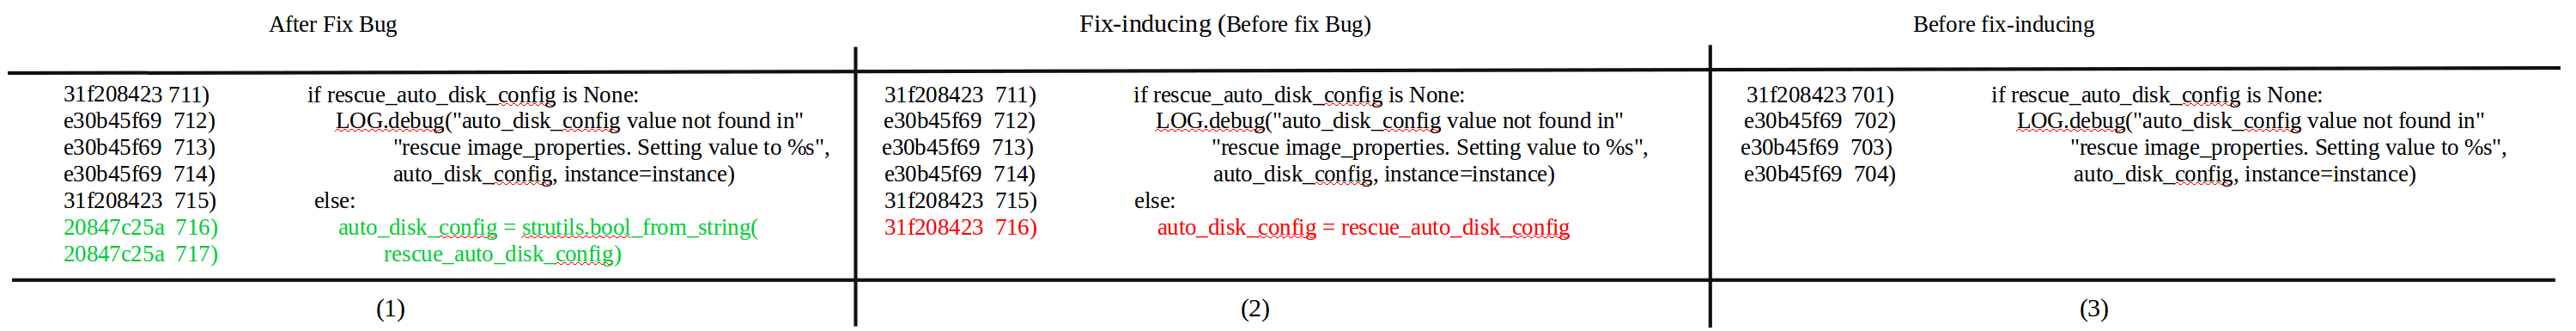
\includegraphics[height=2in, width=7in]{responsible.png}
\caption{Example of a change in which the bug was introduced in the previous commit. More recent versions of the code are on the left.}
\label{fig:1}       % Give a unique label
\end{figure*}


\begin{enumerate}
  \item The code on the left (subfigure \textit{(1)}) is the one written to fix the bug.
  \item The code in the middle (subfigure \textit{(2)}) shows the moment in which the bug was introduced (being \textit{31f08423} the id of change), the previous commit.
  \item The code on the right (subfigure \textit{(3)}) ensures that in previous versions of the file, the bug did not exist.
\end{enumerate}

\begin{figure}[ht]
\centering
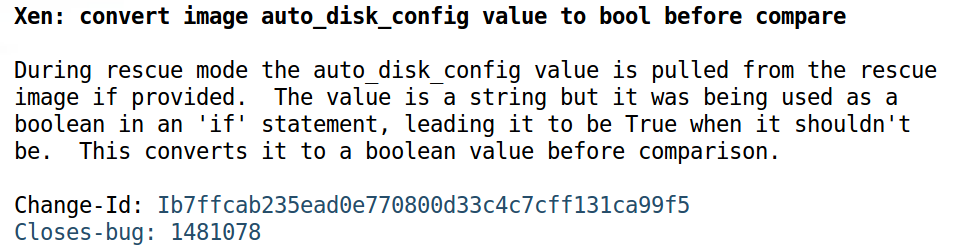
\includegraphics[height=2.4cm]{gerritPrevCommit.png}
\caption{Description of the bug-fix commit for a case in which the previous commit caused the bug.}
\label{fig:2}       % Give a unique label
\end{figure}


According to the description in the log of the commit that fixed the bug (see Figure~\ref{fig:2}), commit \textit{31f08423} was the one where the bug was introduced, as it used a variable as string when a Boolean had to be used, keeping the concordance with the rest of the code. So, in this case, the bug was introduce in the previous commit.


On the other hand, Figure~\ref{fig:3} shows a clear example of a case where the cause of the bug is not to be attributed to the previous commit. In this example, the bug fix commit log (see Figure~\ref{fig:4}) describes that the name of an argument changed when updating the version causing the failure in the software. This change was done because of the new requirements in the software version, and is unrelated to the changes performed in the previous commit. When the modified lines where introduced in the first time, they did not contain the bug.


\begin{figure*}[ht]
\centering
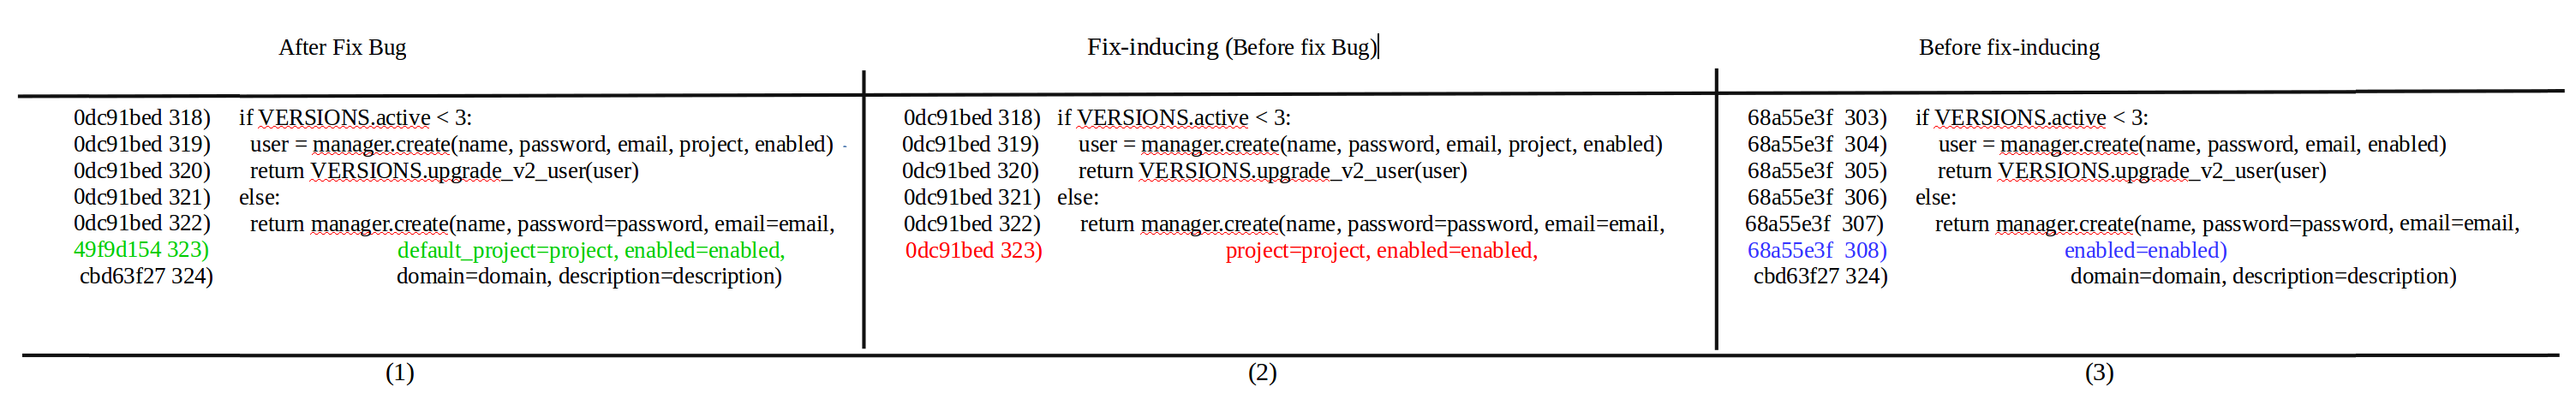
\includegraphics[height=2in, width=7in]{noResponsible.png}
\caption{Example of a change where the previous commit, 0dc91bed, did not insert the bug. More recent versions of the code are on the left.}
\label{fig:3}       % Give a unique label
\end{figure*}

\begin{figure}[ht]
\centering
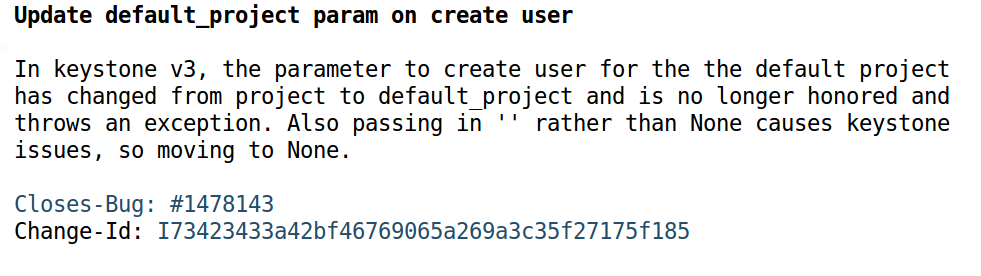
\includegraphics[height=2.4cm]{UpdateFixBug.png}
\caption{Description of the bug-fix commit for a case in which the previous commit did not cause the bug.}
\label{fig:4}       % Give a unique label
\end{figure}

Based on anecdotal evidence like the one presented in Figures~\ref{fig:3} and Figure~\ref{fig:4}, we argue that in projects that are continuously evolving, with an ample developer community, code that before was correct could be buggy at some time. So, changes in other parts
of the code may induce wrong behavior (bugs) in places that were correct in the past. This happens often in situations like changes to the API. In the moment the code ws written, it was correct and the woftware worked fine. Additions of new features or enhancements to the API had as a side effect that the formerly correct code presents a wrong behavior, making the software fail. But in such cases, the source of the error cannot be FIXME assigned to a change performed in the previous commit, as in that moment it referred to a different API.

FIXME: poner esto bien

The goal of this paper is to find if the cause of the bug can be FIXME assigned to the previous commit, understanding that at the time when the previous commit is introduced

not all times the code analyzed was so easy as the code showed in figures \ref{fig:1} and \ref{fig:3}. So the principal aim of this paper to find the responsible of the bug is to know if the previous commits contained buggy code at the moment in which were added/modified or, another change in the software, related to the update of the software and its evolution, caused the bug.

In detail, in this paper we attempt to address the following research question regarding who introduced the bug in the source code:

FIXME: rephrase RQs

\begin{itemize}
    %\item RQ1 : How can tickets which are bug reports be differentiated from those that are not?
     \item RQ1:  How can we know that a change was done to fix a bug in the source code? How can we identify them?
    %\item RQ2:  How often is the bug caused in the previous commit?
     \item RQ2:  When did the previous commit introduce the line with the bug into the source code?
\end{itemize}

The remainder of this paper is structured as follows. Next, we present the current body of knowledge in section~\ref{sec:related}. Section~\ref{sec:methodology} describes the methodology used to identify the moment in which the bug was introduced in the source code, followed by the results obtained after applying our approach to a selection of OpenStack bug fixes in Section~\ref{sec:results}. Section~\ref{sec:discussion} answers the research questions and discusses potential applications and improvements of our approach. After reporting the limitations and threats to validity in Section~\ref{sec:threats}, we draw some conclusions and point out some potential future work in Section~\ref{sec:conclusions}.


\section{Related Work}
\label{sec:related}

The first algorithm to identifying bug-introducing code changes automatically was proposed by Sliwersky et al.~ \cite{sliwerski2005changes}. Currently, it is a well-known algorithm called SZZ, which is based on text differences to discover modified, added and deleted lines between the bug-fix and its previous version. The SZZ algorightm uses the CVS \texttt{annotate} command\footnote{Other versioning systems provide similar functionality to CVS \texttt{anotate}; for instance, git offers \texttt{blame}.} to identify the last commit that touched these lines.

An improvement to the SZZ algorithm is described by Kim et al.~\cite{kim2006automatic}. There the authors used annotation graphs instead of CVS annotation to locate, in the previous versions, the lines affected by modification and deletion. Also, they avoid some false positives by not considering blank spaces, changes in the format or changes in the comments.

Sinha et al. present another technique to identify the origins of a bug in~\cite{sinha2010buginnings}. Their technique is not text-based technique, as the SZZ algorithm, as the authors analyze the effects of bug-fix changes on program dependencies. So, taking into account the semantics of the source code they achieved higher accuracy in identifying the origins of a bug.

The two approaches have some metodological patterns in common:

\begin{enumerate}
  \item They find the differences between the bug-fix version and the previous version of the file to recognize those changes done by the bug-fix commit. 
  \item They look back in the code revision history until they identify which version touched the lines affected in the bug-fix for the last time.
\end{enumerate}

FIXME: This last paragraph should be clarified, and more on papers using the SZZ algorithm! Maybe we should state how many papers in total exist based or using SZZ in Google Scholar.

The SZZ algorithm (and its \emph{successors}) have been widely used in the researc community.
Williams et al. revisited the SZZ algorithm to track bug-inducing changes and identify types of changes~\cite{williams2008szz}. Yang et al. applied SZZ to find what kind of bug-inducing changes are likely to become a great threat after being mared as bug-fix changes
Finally, some bug prediction algorithms are based on SZZ; Kim et al. showed how to classify file changes as buggy or clean using change information features and sour code terms~\cite{kim2008classifying}.

FIXME: maybe talk about my paper with dmg and ahmed, where bugs could be found elsewhere~\cite{german2009change}. There the talk is precisely about those bugs whose origina are elsewhere. Title of the paper: \emph{Change impact graphs: Determining the impact of prior codechanges}

%In addition some tools are based on SZZ too such as \cite{} 
%Finally our idea.

\section{Methodology}
\label{sec:methodology}
%We present our approach to identify how and where a bug was inserted into the source code, causing a later fix. 

All data needed to analyze when the bug was introduced can be obtained from the issue tracking systems and the code review systems used generally by free/open source software (FOSS) projects. In our analysis, we have focused on Launchpad\footnote{\url{https://launchpad.net/}} as issue tracking system, and Gerrit\footnote{\url{https://www.gerritcodereview.com/}} as code review supporting tool, as they are widely used by FOSS projects nowadays, but our methodology should be generalizable to any such tool.

The Launchpad of each project works with issue reports called tickets, which describe bug reports, feature requests, maintenance tickets, and even design discussions. In our study, however, we are only interested in those tickets that have following properties:

\begin{enumerate}
  \item They describe a bug report, and
  \item They have been closed and merged in the code source to fix the described bug.
\end{enumerate}

In these bug reports we can find a comment with the link to Gerrit where the bug was fixed. It is in Gerrit where we can see all the patchsets proposed and the comments done by the reviewers. 

\subsection{Fist Stage: Filtering}
\label{sec:firstStage}

First, we have to identify what issues found in Launchpad are bug reports. This is not a trivial task and is labour intensive as it has to be done manually. As the process is repetitive, we developed a web-based tool\footnote{\url{bugtracking.libresoft.es}} that helps in the classification process. This tool offers all relevant information required to decide if an issue corresponds to a bug report or not. The tool uses information extracted automatically from the project repositories, and offers a web-based interface which allows for collaboration, traceability and transparency in the identification of bug reports.

During the identification of the issues, we have to take into account the next parameters for each ticket:

\begin{itemize}
  \item The title of the issue report
  \item The description of the issue report
  \item The description of the fix commit
  \item The changes to the source code, as sometimes neither the descriptions nor the comments by developers in the Launchpad an Gerrit of each ticket, clarified the underlying ticket. FIXME: what comments?
\end{itemize}

FIXME: aqui podemos poner un pantallazo de la interfaz web.
We can see the web interface of the tool in the image \ref{fig:screenshot}, the left side is used to display the information extracted from Launchapad and Gerrit and the right part is the one in which the users can wirte and classify the ticket into one of the three groups.
\begin{figure}[ht]
\centering
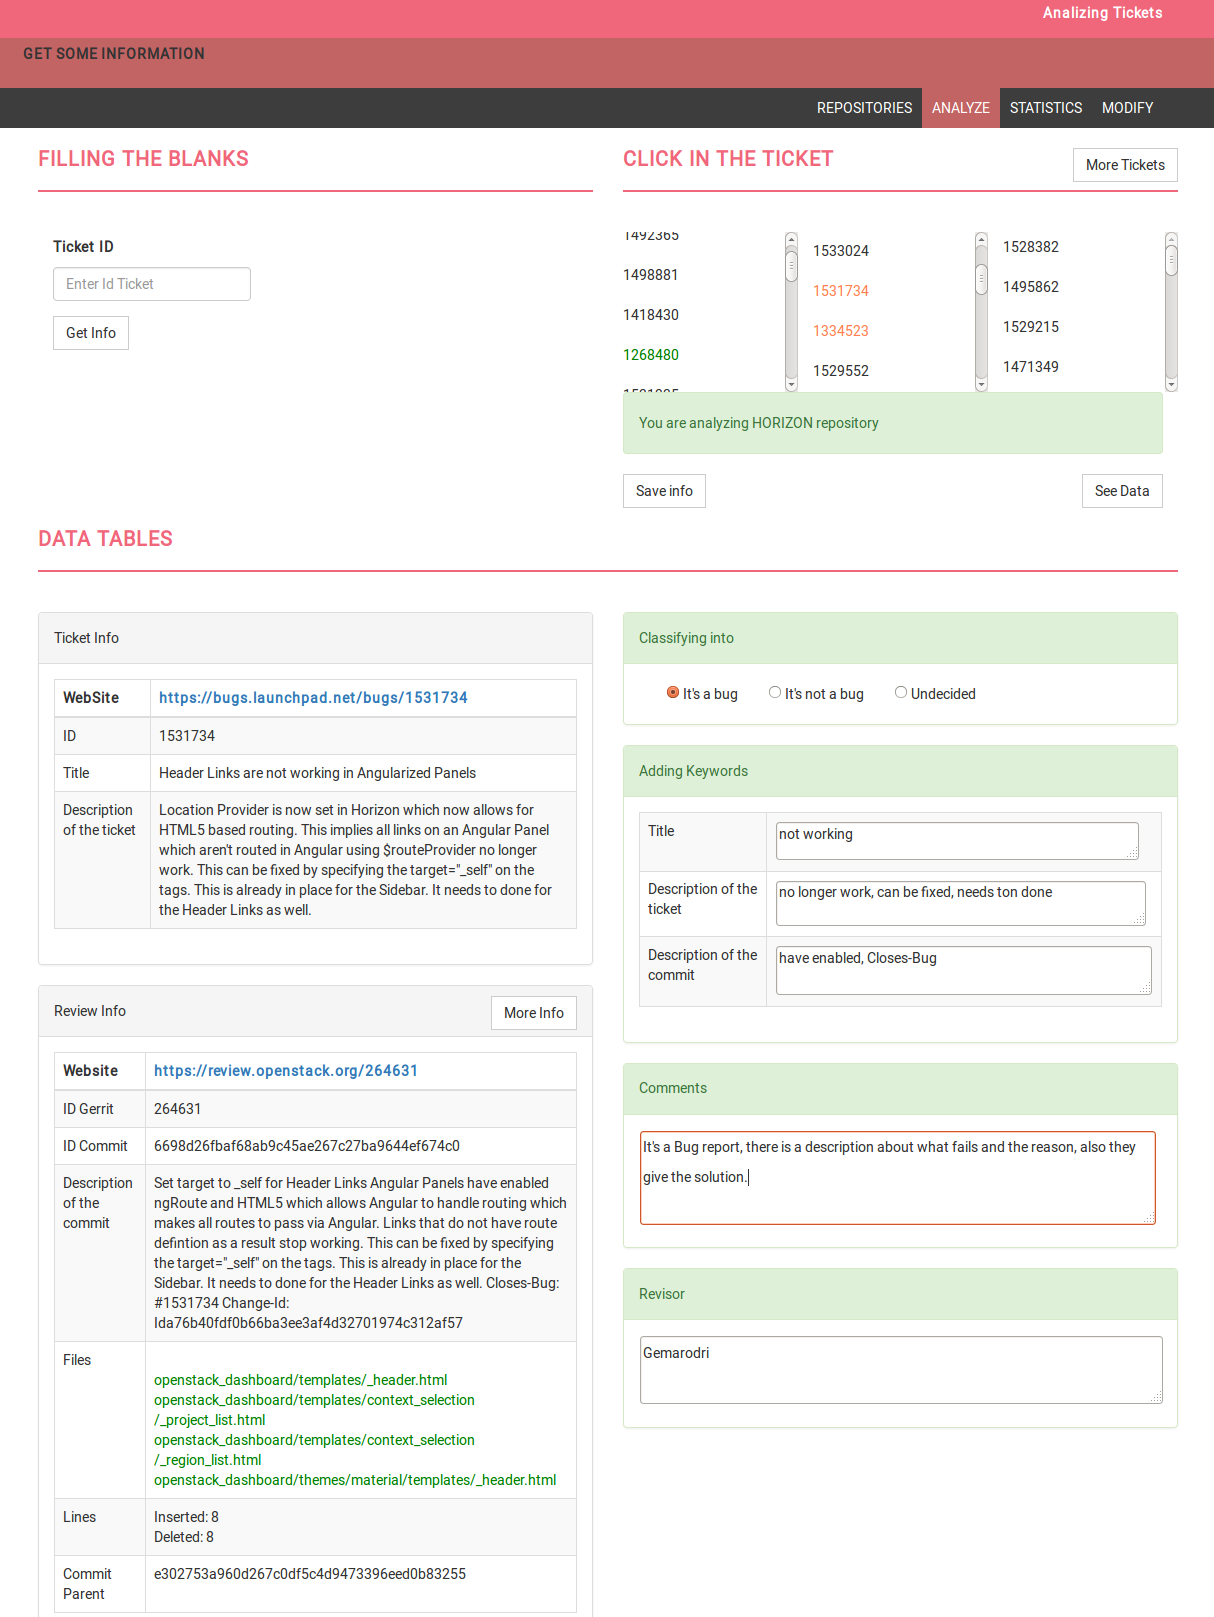
\includegraphics[height=12cm]{index.png}
\caption{Screenshot of the tool used to classify the tickets}
\label{fig:screenshot}       % Give a unique label
\end{figure}

Each ticket was then categorized into one of three following groups:

\begin{enumerate}
  \item Group 1 (\textit{Bug Report}): The ticket describes a bug report.
  \item Group 2 (\textit{Not Bug Report}): The ticket describes a feature, an optimization code, changes in test files or other not bug reports.
  \item Group 3 (\textit{Undecided}): The ticket presents a vague description and cannot be classified without doubts.
\end{enumerate}

From the experience of analysing a small number of tickets, we agreed on following four criteria: 

\begin{enumerate}
    \item When the ticket title described the program as not working as expected, our criteria indicated that it was a bug report. 
    \item When the title described optimization, deletion of a dead code or the implementation of new characteristics, we agreed not to classify it as a bug report because there is no failure. 
    \item When the ticket title described that updates were required, the ticket is a bug report. We consider all tickets that require updating as bug reports, because updating a software hints to the software not operating as expected. 
    \item When only test files are affected in a ticket, we classified it as not being a bug report. Test files in a ticket were not be analyzed, as we consider they are not a core part of the software and are used as a testing method to determine whether the code is fit for use. When the bug exclusively lies in a test file, the ticket was not considered as bug report because the software still works as expected, only test fails. FIXME: no se repiten las frases?
\end{enumerate}

Sometimes we were unable to answer all the questions due to having insufficient data or because of the complexity of the issue. In this case, the ticket was classified into the \textit{Undecided} group.

\subsection{Second Stage: Who caused the Bug?}
\label{sec:secondStage}

The next part is focused on analyzing the previous commit exclusively in the \textit{Bug Report} group to identify which line contained the bug and why the software failed, keeping in mind the context of the project. For that, we had to analyze the lines involved in the bug fix and in the \emph{parent} commit of the bug fix commit, being sure that the lines were added,inserted or modified in the previous commit. This way, we can be sure that we are looking the correct change, because some times although the commit added many lines, if you look the code before the commit you can check that some of the lines added was there, and in that case, is a false positive where the previous commit didn't cause the bug. FIXME: aclarar este parrafo! 

The analysis was done manually. We used \textit{git blame} to see the previous commit for each line of the involved file. Also, we used \textit{diff} to see the differences between the two files, in our case as the file is going to be the same, between the file in two different moments in the control version system.

The procedure for each file involved in a bug fix is as follows:

\begin{enumerate}
  \item git checkout \textit{commit that fixed the bug}, git blame \textit{file involved}. In this step we can see the lines added, modified or deleted by the commit that fixed the bug.
  \item git checkout \textit{parent of commit that fix the bug}, git blame \textit{file involved}. In this step we can see the previous commits for the different lines touched in the fixed bug.
  \item git checkout \textit{parent of previous commit}, git blame \textit{file involved}. With this step we can ensure that the previous commit inserted these lines.
\end{enumerate}

Finally we need to discard some noise presents in our final results according to the responsibility of the previous commit inserting the bug in the code source. Due to they were not responsible for cause the bug, we delete those previous commit which presents the following criteria:

\begin{itemize}
    \item Blank lines
    \item Format changes
    \item Copied lines
    \item Changes in the comment.
    \item Updates in the version of a file. 
\end{itemize}


\section{Evaluation}
\label{sec:evaluation}

We validate our methodology analyzing 459 tickets from OpenStack. OpenStack is a cloud computing platform with a huge developing community (more than 5,000 developers) and significant industrial support from several major companies such as Red Hat, Intel, IBM, HP, etc. OpenStack was particularly of interest because of its continuously evolving due to its very active community. Currently it has more than 233,000 commits with more than 2 million lines of code \footnote{\url{http://activity.openstack.org/dash/browser/}}. All its history is saved and available in a version control system, as well as its issue tracking system (Launchpad\footnote{\url{https://launchpad.net/openstack}}) and the source code review system (Gerrit\footnote{\url{https://review.openstack.org/}}).

OpenStack is composed by 9 projects, but we only focused in four of them: Nova, Cinder, Neutron and Horizon. As can be seen from Table~\ref{tab:OpenStack}, these projects have been very active during their entier history, and in the last year.

\begin{table}[htb]
\centering
%\begin{center} {\footnotesize
\begin{tabular}{lrr}
\toprule[0.3mm]%{\smallskip}
  & All History  & Last Year (2015) \\\hline
Nova    \kern 1pc & 14,558 & 3,283 \\
Fuel    \kern 1pc & 9,139 & 5,123 \\
Netron  \kern 1pc & 8,452 & 3,855 \\
Horizon \kern 1pc & 4,871 & 1,994 \\
Cinder  \kern 1pc & 4,556 & 1,832 \\
Keystone\kern 1pc & 4,874 & 1,795  \\
Heat    \kern 1pc & 6,395 & 2,372  \\
Glance  \kern 1pc & 2,651 & 723 \\
Tempest \kern 1pc & 4,141 & 1,312 \\
\bottomrule[0.3mm]
\end{tabular} %}
\caption{ Commits per Project in OpenStack}
\label{tab:OpenStack}

%\end{center}
\end{table}

In this four projects we analyzed the relationship of bug fixes with their previous commits. In order to identify the moment in which the bug was injected into the source code. The first stage we did automatically using the tool and a double bind between three researchers, three PhD student  included me. The second stage was done manually and only me was involved analyzing this relationship. %that, we extract a total of 459 tickets from this projects, in which we should be sure that the bug fixes come from a bug report, because two of five issues are misclassified \cite{herzig2013s} and this should cause bias in our final results.

\section{Results}
\label{sec:results}

We extracted a total of 459 different tickets from the Launchpad of the four principal projects in OpenStack, 125 tickets from Nova, 125 tickets from cinder, 125 tickets from Horizon and 84 tickets from Neutron. These tickets first, were analyzed to identify those ones which were real bug reports. And secondly, each file was analyzed to obtain which previous commit inserted the bug causing the failure of the system and reporting the bug report. 

\subsection{Fist Stage}
\label{sec:resultsFS}

We classify a total of 459 tickets using the tool. In 417 of the tickets, we used double bind analysis, and only those tickets classified as bug report by two of us, were considered in the next stage to analyze the relevance of their previous commits.

The table \ref{tab:2} shows the percentage of each researcher after analyzing the tickets, and the number of tickets classified identically by two different researchers. Obtaining that the researchers R1 and R2 had a similar data in their results, whereas research R2 got results significantly different with a higher number of tickets classified as Bug Report.
 
Finally, the researchers identified in the same way 292 tickets, that is, their results matched in a 70\% of the cases. Obtaining 209 tickets classified as Bug report, 74 tickets classified as Not Bug Report and 9 tickets classified as Undecided.

\begin{table}
\centering
%\begin{center} {\footnotesize
\begin{tabular}{lrrrr}
\toprule[0.3mm]%{\smallskip}
  & Bug Report & Not Bug Report & Undecided & Total \\\hline
R1  & (184) 55\% & (115)34\% & (35) 11\% & 334 \\
R2  & (188) 76\% & (54)22 \% & (7) 3\% & 249 \\
R3 & (188) 56\% & (116) 35\% & (30) 9\% & 334 \\
Finally & (209) 72\% & (74) 25\% & (9) 3\% & 292 \\
\bottomrule[0.3mm]
\end{tabular} %}
\caption{ Statistics of each researcher in the classification}
\label{tab:2}
%\end{center}
\end{table}

Also we had measured the concordance in the classification of each developer according to the project analyzed. The table \ref{tab:3} shows that the concordant got between all the three research was very similar, around a 70\%. Furthermore, the concordance form each researcher with the rest always was up to 60\%. 

\begin{table}[htb]
\begin{center} {\footnotesize
\begin{tabular}{lrrrrr}
\toprule[0.3mm]%{\smallskip}
  & Nova & Cinder & Horizon & Neutron & Total\\\hline
R1\&R2   & (44) 70\% & (40) 77\%  & (37) 60\% & -        & 68\% \\
R1\&R3   &  -        & (46) 73\%  & (48) 76\% & (26) 62\% & 71\% \\
R2\&R3   & (41) 66\% & (10) 100\% & -         & -        &  71\% \\
\bottomrule[0.3mm]
\end{tabular} }
\caption{ Concordance between each developer in each repository}
\label{tab:3}
\end{center}
\end{table}



\subsection{Second Stage}
\label{sec:resultsSS}

At this stage, we analyzed the 209 we got a list with all the previous commits and we were be able to classified the previous commit/s as Responsible, Not Responsible or Undecided, taken into account that the bug could be inserted in different lines of different commits, but not everyone had to be responsible for the commit, sometimes the previous commit copied lines from its previous commit or inserted comments and blank spaces. In fact, the responsible can be only one of them, more than one or maybe none.

We identified a total of 348 previous commits which can be responsible for inserting the line containing the bug. After analyzing the Bug Reports and their previous commits and discarded 40 of them because were noise, Table \ref{tab:responsability}, we got that 152 previous commit were responsible to cause the bug whereas 114 previous commit had not any responsibility in the failure of the system, and only in 42 previous commits we were unable to identify the cause of the bug.

\begin{table}[htb]
\begin{center} {\footnotesize
\begin{tabular}{lrr}
\toprule[0.3mm]
  & \multicolumn{1}{c}{Before} & \multicolumn{1}{c}{After} \\
  & \multicolumn{1}{c}{Deleting Noise} & \multicolumn{1}{c}{Deleting Noise} \\\hline
\raisebox{1ex}{Responsible} & 152 & 152 \\[0ex]
\raisebox{1ex}{Not responsible} & 154 & 114 \\[0ex]
\raisebox{1ex}{Undecided} & 42 & 42 \\[0ex]
\bottomrule[0.3mm]
\end{tabular} }
\caption{ Responsibility of each previous commit before and after deleting the noise in the results}
\label{tab:responsability}
\end{center}
\end{table}

Furthermore, focusing on how many previous commits presented each Bug Report, we obtained that 131 had one previous commit implicated, whereas 58 had more than one previous commit implicated in their file/s. According to Table \ref{tab:secondStage}, from the 131, we obtained that 65 of them inserted the bug, but 30 of them were not responsible in the failure of the system. And from the 58 which had more than one previous commits, we obtained in total 189 previous commit, where 86 of them were responsible and 82 were not responsible. %Probably, the bug was inserted in different lines of different commits, but not everyone has to be responsible for the commit, sometimes the previous commit copied lines from its previous commit or inserted comments and blank spaces. After the analysis the responsible can be only one of them, more than one or maybe none. 

\begin{table}[htb]
\begin{center} {\footnotesize
\begin{tabular}{lcc}
\toprule[0.3mm]
  & \multicolumn{1}{c}{One previous } & \multicolumn{1}{c}{More than one previous} \\
  & \multicolumn{1}{c}{commit} & \multicolumn{1}{c}{commit} \\\hline
\raisebox{1ex}{Responsible}     & 65 & 86 \\[0ex]
\raisebox{1ex}{Not responsible} & 30 & 82 \\[0ex]
\raisebox{1ex}{Undecided}       & 36 & 11 \\[0ex]
\bottomrule[0.3mm]
\end{tabular} }
\caption{ Probability of cause the bug depending on how many previous commits had the bug report}
\label{tab:secondStage}
\end{center}
\end{table}

Also, we looked the distribution of the previous commit in each Bug Report, Table \ref{tab:secondStage2}, we observed that the most common distribution in the relationship between previous commit and bug report is one previous commit per Bug Report, following by the second common distribution, two previous commit per Bug Report.

\begin{table*}[htb]
\begin{center} {\footnotesize
\begin{tabular}{lccccc}
\toprule[0.3mm]
  & \multicolumn{1}{c}{One previous} & \multicolumn{1}{c}{two previous} & \multicolumn{1}{c}{three previous} & \multicolumn{1}{c}{four previous} & \multicolumn{1}{c}{+five previous}\\
  & \multicolumn{1}{c}{commit} & \multicolumn{1}{c}{commit} & \multicolumn{1}{c}{commit}& \multicolumn{1}{c}{commit}& \multicolumn{1}{c}{commit}\\\hline
\raisebox{1ex}{Neutron} & 11 & 3 & 2 & 2 & 0 \\[0ex]
\raisebox{1ex}{Horizon} & 39 & 8 & 3 & 2 & 4 \\[0ex]
\raisebox{1ex}{Nova} & 44 & 5 & 2 & 4 & 4 \\[0ex]
\raisebox{1ex}{Cinder} & 37 & 9 & 6 & 2 & 2\\[0ex]
\raisebox{1ex}{Total} & 131 & 25 & 13 & 10 & 10\\[0ex]
\bottomrule[0.3mm]
\end{tabular} }
\caption{ Distribution of number of previous commit per Bug Report in each project}
\label{tab:secondStage2}
\end{center}
\end{table*}

Finally we wanted to know the responsibility practiced by each previous commit in the failure of a system, in other words, we were interested in analyze from those cases where exists more than one previous commit, how many of them inserted the bug in the code source, Table \ref{tab:secondStage3}. We obtained that in 8 Bug Reports all the previous commits were responsible, in 30 Bug reports at least one of their previous commit caused the bug and in 11 bug report none of their previous commits inserted the bug.

\begin{table*}[htb]
\begin{center} {\footnotesize
\begin{tabular}{lccccc}
\toprule[0.3mm]
   & \multicolumn{1}{c}{two previous} & \multicolumn{1}{c}{three previous} & \multicolumn{1}{c}{four previous} & \multicolumn{1}{c}{+five previous} & \multicolumn{1}{c}{Total}\\
  & \multicolumn{1}{c}{commit} & \multicolumn{1}{c}{commit}& \multicolumn{1}{c}{commit}& \multicolumn{1}{c}{commit}\\\hline
\raisebox{1ex}{All Responsible}          & 4 & 3 & 0 & 1 & 8\\[0ex]
\raisebox{1ex}{At least one responsible} & 9 & 7 & 5 & 9 & 30\\[0ex]
\raisebox{1ex}{None Responsible}         & 4 & 2 & 4 & 1 & 11\\[0ex]
\raisebox{1ex}{Undecided}                & 1 & 0 & 1 & 0 & 2\\[0ex]
\bottomrule[0.3mm]
\end{tabular} }
\caption{ Probability of cause the bug depending on how many previous commits had the bug report}
\label{tab:secondStage3}
\end{center}
\end{table*}


\section{Discussion}
\label{sec:discussion}


\fbox{\begin{minipage}{25em}

\textbf{RQ1: Using all the information available in the bug tracking system and code review system related a fix-bug, we have obtained that this fix-bug were real Bug Reports in a 72\% of the tickets analyzed} 
\end{minipage}}

\fbox{\begin{minipage}{25em}
\textbf{RQ2: We have confirmed that 50\% of the previous commits analyzed caused the failure in the system, whereas the 37\% of them didn't injected any bug in the code source } 
\end{minipage}}
FIXME: Debería hablar sobre los siguientes puntos:
\begin{enumerate}
 \item No todos los casos son tan claros como los mostrados en los ejemplos ....
 \item Casuistica del common juidment
 \item Hemos sido conservadores
 \item Hemos utilizado la herramienta porque es un proceso complicado
\end{enumerate}

Once we have all the tickets analyzed by diferents researchers who have used a double blind, how to proceed if there are discordances between them:

\begin{enumerate}
  \item Should they discuss after their analysis to reach a better classification?, Should the tool provide this?
  \item Does the Bug report only the same ticket classified as Bug report for all the researchers?
\end{enumerate}

How to proceed if looking for the responsibility of a bug when only added lines are inserted? And we are talking about a bug report not a new feature, these kinds of cases use to be when a researcher forgot check some case inside a function.
\begin{enumerate}
\item Is responsible the function where these lines are content?
\item Is responsible the last commit that modify something in the function?
\end{enumerate}


\section{Threats to validity}
\label{sec:threats}
%The limited sample size of tickets used in this research is the major threat to its validity. %It may happen, that only with 100 seemingly random tickets, there may be a prior unknown tendency. This is in fact similar to~\cite{sliwerski2005changes}, where the trend indicates that most bugs are fixed on Fridays.
The size of the tickets extracted form the Launchpad is medium, but doing the analysis manually we are sure that the results present in this paper are valid, being sure that the previous commits classified as not responsible, they are. 

Although, we understand that the model presented has some threats, external and internal, that make our model not 100\% valid. The internal threats related to the researchers that have conducted the study are following:

\begin{itemize}
    \item We have not taken into account errors that have been classified into \textit{Undecided}, and probably we are lost some real bug reports belonging this group .
    \item There could be some lax criteria involving the subjective opinion of the researchers.
    \item The researchers are not experts in OpenStack, and our inexperience may have influenced the results of the analysis.
    \item We are only using part of the information that the ticket provides, like comments and text. There could be a recognized pattern in the data, unknown at first sight, that involves other parts of the information.
    \item Although we use a random script to extract the tickets reported in during the last year, 2015, from the launchpad, in this year could be some bias unidentified.
    \item In case of the researchers didn't find the information to know if the previous commit inserted the bug or in contrast, it was caused by the evolution of the software. They keep the traditionalist thought, classify these previous commits are responsible.
\end{itemize}

The external threats, related to the case of the project, are following:

\begin{itemize}
    \item The word \textit{bug} is continuously mentioned in the description and commit of a ticket even when we found it is not an error. This could lead to the incorrect classification during the reviewing process.
    \item Some tickets are not explicitly described, which could increase the percentage of \textit{Undecided}. This is especially true if the reviewers are not from OpenStack.
    \item OpenStack is a special project put down a constant evolution due to their active community of developers. Maybe, in other projects with less commits per year the statistics about the responsibility of previous commit change.
\end{itemize}
FIXME: Anñadir un link con la web en la que pondré todos los datos y scripts utilizados para los datos.

\section{Conclusions and Future Work}
\label{sec:conclusions}
The empirical experiment carried out in OpenStack, supported that the current premise assumed does not hold for a large fraction of the analyzed bugs, because around the 40\% of the previous commits were not responsible inserting the bug.
With our results we can identify which ones are real changes that introduced the bug, and this could be useful to improve the accuracy of those tools developed to prevent bugs. Also, the software developers stand to benefit from identifying where the bug was inserted, improving their methodology.
%How to plan to apply the knowledge in a way that can benefit software engineers.
%What are the anticipated contributions of the work?  How will you evaluate them to demonstrate usefulness?

A final field in our future work concerns the full automation on the methodology could developer an automatic classifier base on the idea that not all the previous commit injected the bug. Another interesting investigation could perform the same empirical study in a project with a community less active, to can prove if our idea is fulfill in other projects.

%ACKNOWLEDGMENTS are optional
\section{Acknowledgments}
We thank Dorealda Dalipaj and Nelson Sekitoleko, two PhD students in our research team, that participated in the process of classifying bug reports. We also want to express our gratitude to Bitergia\footnote{\url{http://bitergia.com/}} for the OpenStack database and the support they have provided when questions have arised. 
Finally, we would like to acknowledge the Spanish Government because all authors are funded in part by it, through project TIN2014-59400-R.

\nocite{*}
%
% The following two commands are all you need in the
% initial runs of your .tex file to
% produce the bibliography for the citations in your paper.
\bibliographystyle{abbrv}
\bibliography{sigproc}  % sigproc.bib is the name of the Bibliography in this case
% You must have a proper ".bib" file
%  and remember to run:
% latex bibtex latex latex
% to resolve all references
%
% ACM needs 'a single self-contained file'!
%
%APPENDICES are optional
%\balancecolumns
\end{document}
